\chapter{Contexte générale du projet}

    \section*{Introduction}
        Dans ce chapitre, nous allons mettre notre projet en contexte, c'est-à-dire definit l'organisme d'acceuil, problématique, état d'art et finalement solution proposée, donc en résumé, notre travail dans ce projet est une etude des radiographies médicales plus clairement la classification de ces derniers suivant une list de diagnostiques, mais plus important encore, notre objectif est de répondre à la question "pouvons-nous obtenir de bons résultats à partir d'une petite base de donées?".

    \section{Organisme d'acceuil}

        \subsection{CHU Mohammed VI de Marrakech}
            \begin{figure}[h]
                \centering
                
\includegraphics[width=0.3\textwidth]{icon_chu.png}\label{fig:chu}
                \caption{Icone du CHU}
            \end{figure}
            Le Centre Hospitalier Universitaire Mohammed VI de Marrakech joue un rôle  majeur et important dans l’offre de soins non seulement dans la région de Marrakech-Safi, mais  dans toute la partie sud du Royaume.

            Il se compose de quatre hôpitaux et deux centres, d’une capacité de 1548 lits dont :
            \begin{enumerate}
                    \item L’Hôpital IBN TOFAIL à vocation médico-chirurgicales d’une capacité de 409 lits.
                    \item L’Hôpital MERE – Enfant à vocation gynéco-obstétricale et pédiatrique d’une capacité de 247 lits.
                    \item L’Hôpital IBN NAFIS à vocation psychiatrique d’une capacité de 220 lits.
                    \item L’Hôpital AR-RAZI à vocation médico-chirurgicales d’une capacité de 586 lits.
                    \item Le Centre d'hématologie-Oncologie : 86 lits.
                    \item Le Centre de recherche clinique.
            \end{enumerate}

            \subsubsection{Chiffres clés de production e CHU}
            Le Centre Hospitalier Mohammed VI est un établissement public doté de la personnalité morale et de l’autonomie financière. Il est soumis à la tutelle du Ministère de la Santé. Il a été crée en vertu de la Loi 82.00 promulguée par le Dahir 1.01.206 du 10 Joumada II 1422 (30 août 2001) modifiant et complétant la loi 37.80 relative aux centres hospitaliers, promulguée par le Dahir 1.82.5 du 30 rabia I (15 janvier 1983).

        
            \subsubsection{Service de radiologie mère-enfant}\label{service_radio}
            Notre travail a été mené au sein du service de radiologie de l’hopitale mère-enfant , qui se spécialise dans l’imagerie médicale pédiatrique et gynécologique , avec un équipement qui comprend la majorité des diverses outils d’imagerie médicale.
            
            \vspace{3mm}
            \begin{multicols}{2}
                \begin{itemize}
                    \item[$\bullet$] Scanners.
                    \item[$\bullet$] Appareil de radiologie télécommandée.
                    \item[$\bullet$] Appareils de radiologie conventionnelle.
                    \item[$\bullet$] Amplificateurs de brillance.
                    \item[$\bullet$] Echo-cardiographies.
                    \item[$\bullet$] Echo-doppler couleur.
                    \item[$\bullet$] Echographes.
                    \item[$\bullet$] Ostéodensitométre.
                    \item[$\bullet$] Appareils de radiologie mobile.
                    \item[$\bullet$] Mammographes.
                    \item[$\bullet$] Systèmes de numérisation par écran ERLM.
                \end{itemize} 
            \end{multicols} 
            \vspace{3mm}

        \subsection{Collaborateurs}\label{Collaborateurs}
            \begin{itemize}[label=$\bullet$]
                \item Professeur et chef de service de radiologie médicale mère-enfant:\newline
                Superviser les autres collaborateurs chargés de la collecte de données et suivre l'avancement du projet étape par étape.
                \item Thésard de médecine:\newline
                Collection de radiographies pulmonaires pédiatriques.
                \item 8 Résidents médecins radiologue seniors et juniors:\newline
                4 résidents juniors\newline
                4 résidents séniors \newline
                Diagnostic et remplissage des données concernant les clichés déjà collectés.
                \item Techniciens radiologues:\newline
                Fournir les radiographies d'intérêt pour notre projet.
            \end{itemize}


    \section{Contexte générale du projet}

        \subsection{Problématique}
            La radiologie médicale est considérée comme le domaine de la médecine qui a le plus bénéficié de l'IA  vue la diversité des zones de son application, voici une liste non exhaustive de ces applications:
            \vspace{3mm}
            \begin{itemize}
                \item[$\bullet$] automatisation de la détection des images pathologiques.
                \item[$\bullet$] la détection des lésions incidentes, non recherchées « a priori ».
                \item[$\bullet$] fiabilisation de l’interprétation des images.
                \item[$\bullet$] identification des motifs, autorisant la classification de lésions.
                \item[$\bullet$] établissement des comptes rendus uniformisés.
                \item[$\bullet$] traitement de larges cohortes d’images radiologiques. 
            \end{itemize}
            \vspace{5mm}

            Dans notre étude on va se concentrer sur l’automatisation de détection d’anomalies ou de constatations radiologiques sur des clichés numérisés de radiographie thoracique standard chez la population pédiatrique.

            La plupart des études d'IA pour l'interprétation des radiographies thoraciques sont appliquées sur des images de population adulte ( tranche d'âge supérieure à 18 ans) avec une couverture de la vaste majorité des anomalies radiologiques et des pathologies thoraco-pulmonaires.

            Alors qu’au niveau pédiatrique, ils se sont concentrés sur un nombre limité de pathologies ou d'anomalies radiologiques sans faire de progrès significatifs en raison de l'absence de  jeu de données  pédiatriques à grande échelle.

            \subsubsection{Procédure de détection des anomalies par les radiologues sur les radiographies thoraciques}
            \paragraph*{Rappel :Formation de l’image radiologique}
            \begin{enumerate}
                \item Tube de Coolidge produit un faisceau de RX
                \item Faisceau incident et homogène de RX
                \item Patient atténuant le faisceau de RX
                \item Faisceau sortant (transmis) de RX hétérogène: image radiante
                \item Appareil de détection reçoit le faisceau transmis
            \end{enumerate}
            La radiographie thoracique est un outil très performant en médecine clinique et savoir interpréter correctement une radiographie thoracique est indispensable aux cliniciens.
            \begin{multicols}{2}
                \begin{itemize}[label=$\bullet$]
                    \item Cadre osseux
                    \item Parties molles
                    \item Diaphragme
                    \item Coeur
                    \item Médiastin
                    \item Hiles
                    \item Poumon
                \end{itemize}
            \end{multicols}
            \begin{figure}[h]
                \centering
                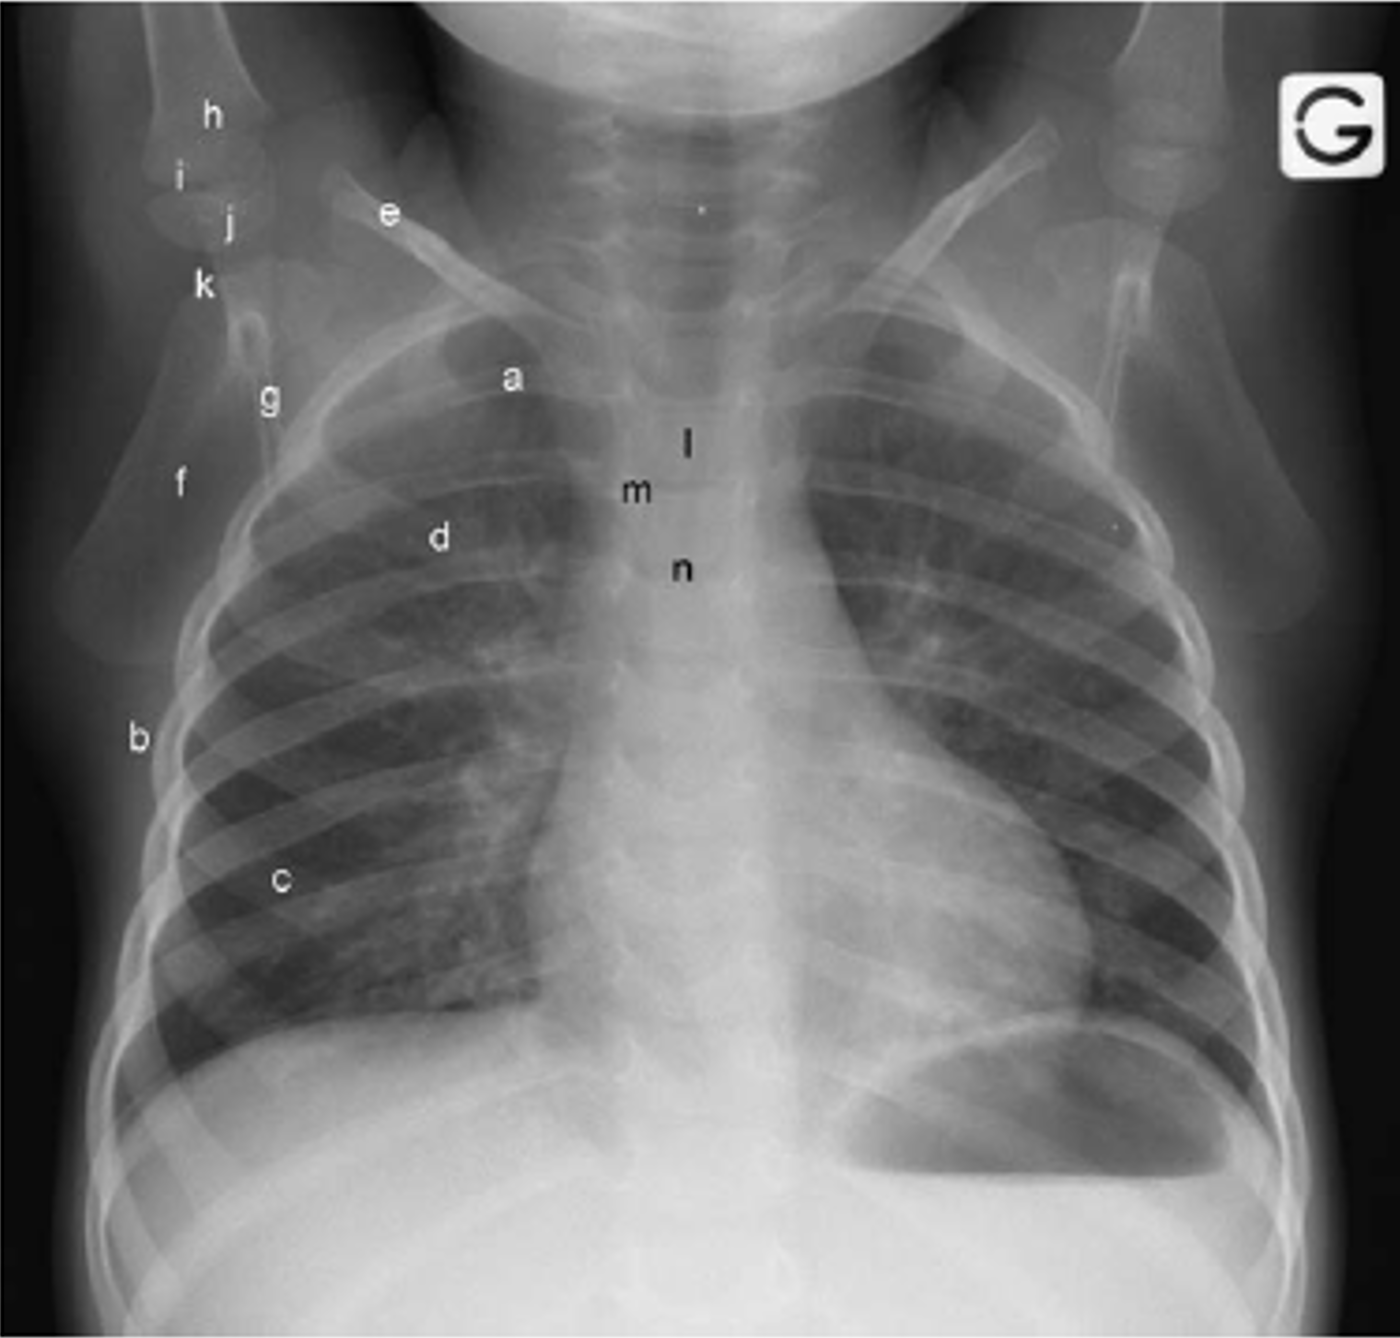
\includegraphics[width=0.4\textwidth]{thorax_osseux.png}
                \caption{Thorax osseux. a. Arc postérieur de la côte; b. arc moyen de la côte ; c. arc antérieur de la côte ; d. extrémité antérieure de la côte; e. clavicule vue en enfilade avec nouure centrale (bras relevés); f. omoplate; g. épine de l'omoplate; h. métaphyse humérale ; i. cartilage de conjugaison; j. épiphyse humérale ; k. cavité glénoïde; l. corps vertébral; m. pédicules; n. disque intervertébral.
                }\label{fig:thorax}
            \end{figure}
           
            \begin{figure}[H]
                \centering
                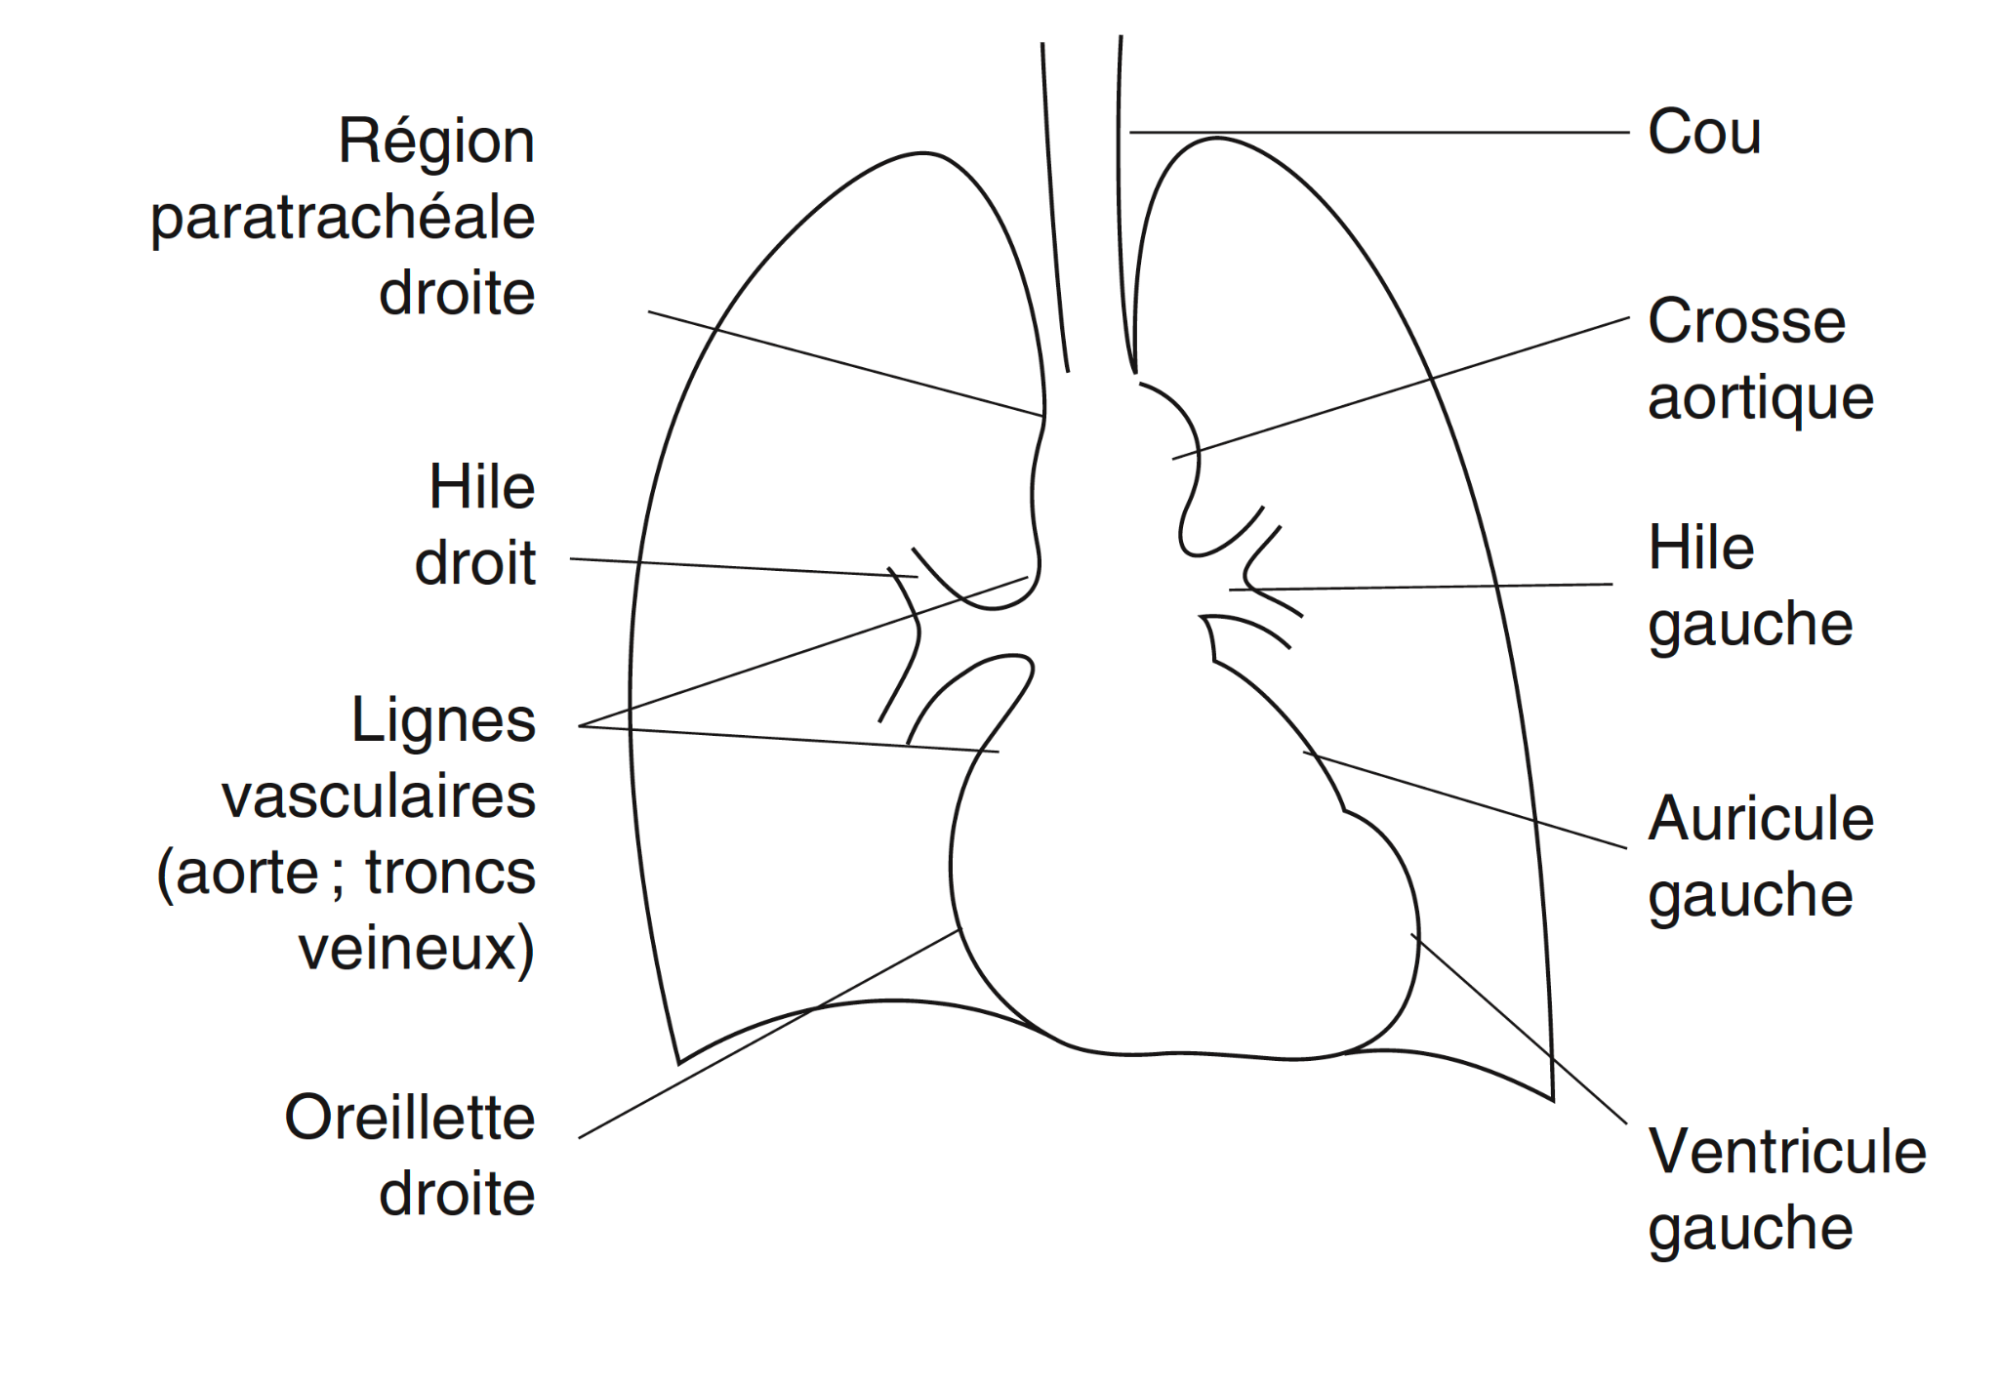
\includegraphics[width=0.6\textwidth]{dia_mediastinal.png}
                \caption{Diagramme des structures médiastinales à analyser sur une Radiographie thoracique PA}\label{fig:mediastinal}
            \end{figure}
            \subsubsection{Les differences radio anatomiques entre les clichés pédiatriques et adultes}

            Sept différences entre la radiographie thoracique d'un nourrisson et celle d'un adulte.

            \begin{figure}[H]
                \centering
                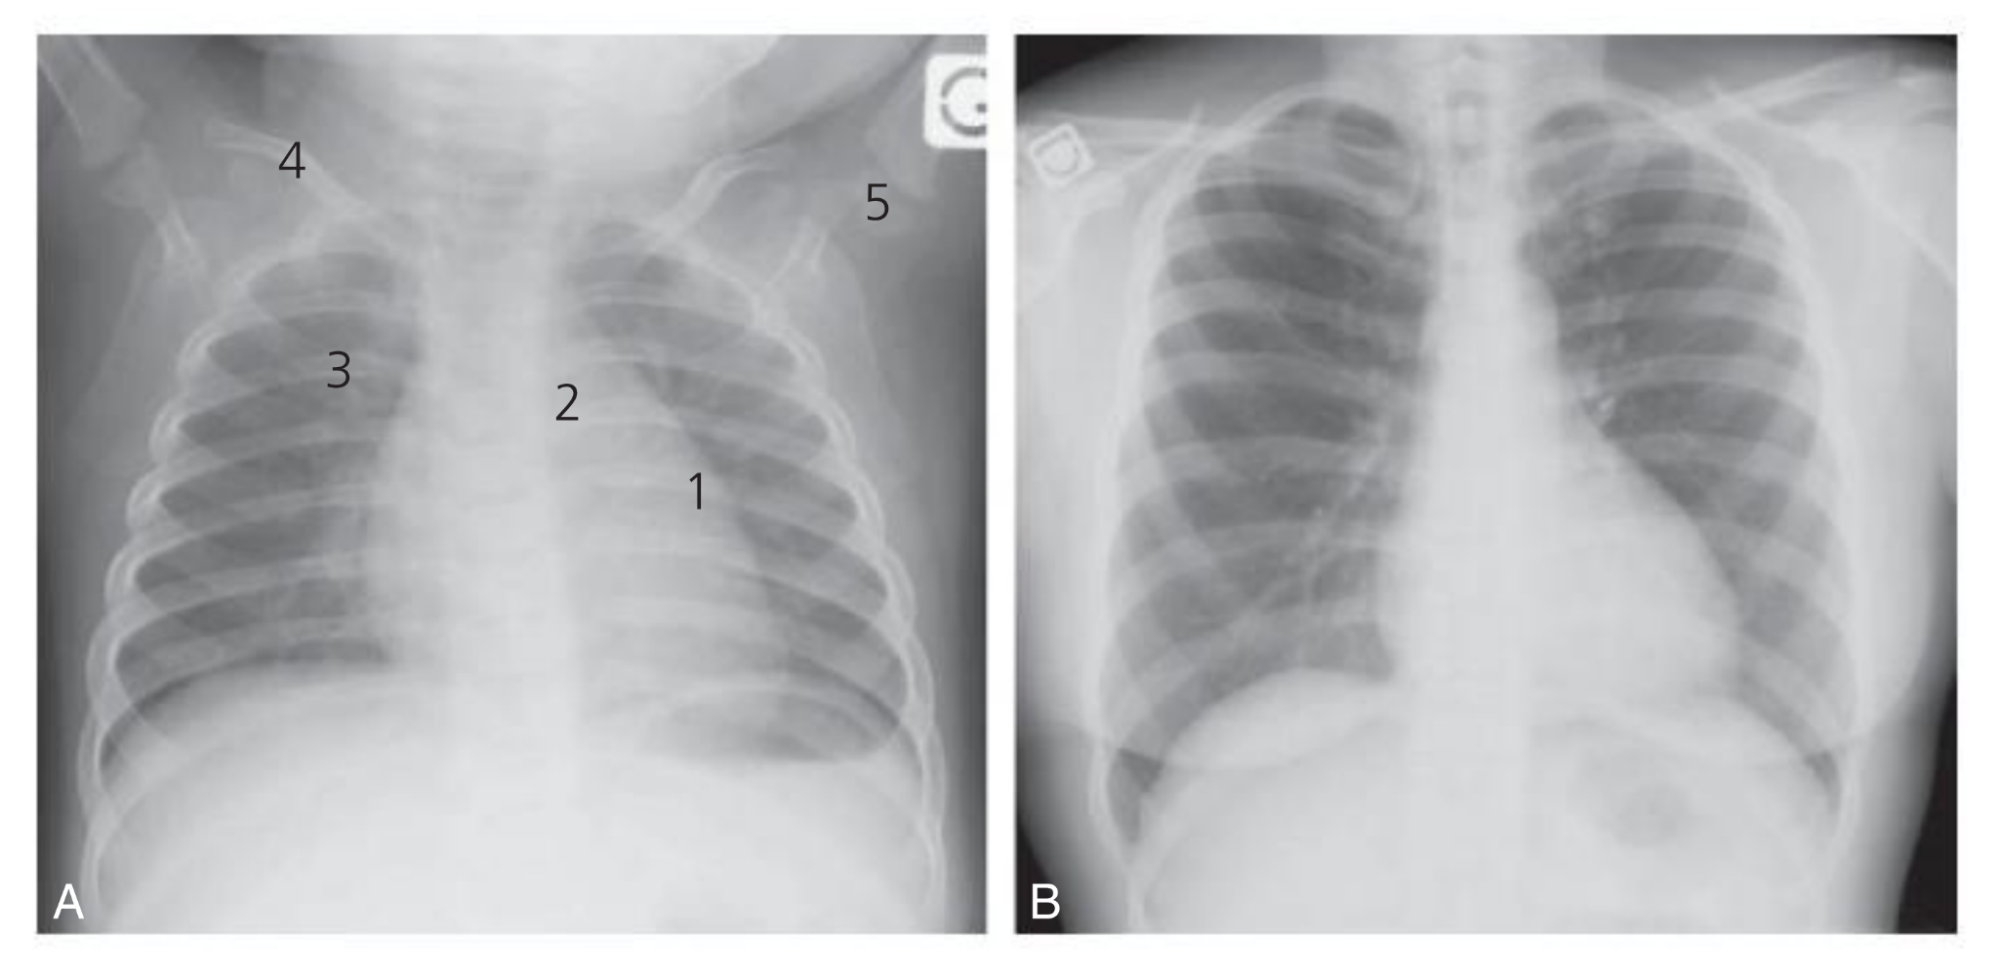
\includegraphics[width=0.6\textwidth]{differences.png}
                \caption{Les différences radio-anatomiques entre l’adult et l’enfant}\label{fig:differences}
            \end{figure}

            \begin{enumerate}
                \item présence du thymus:
                \begin{figure}[H]
                    \centering
                    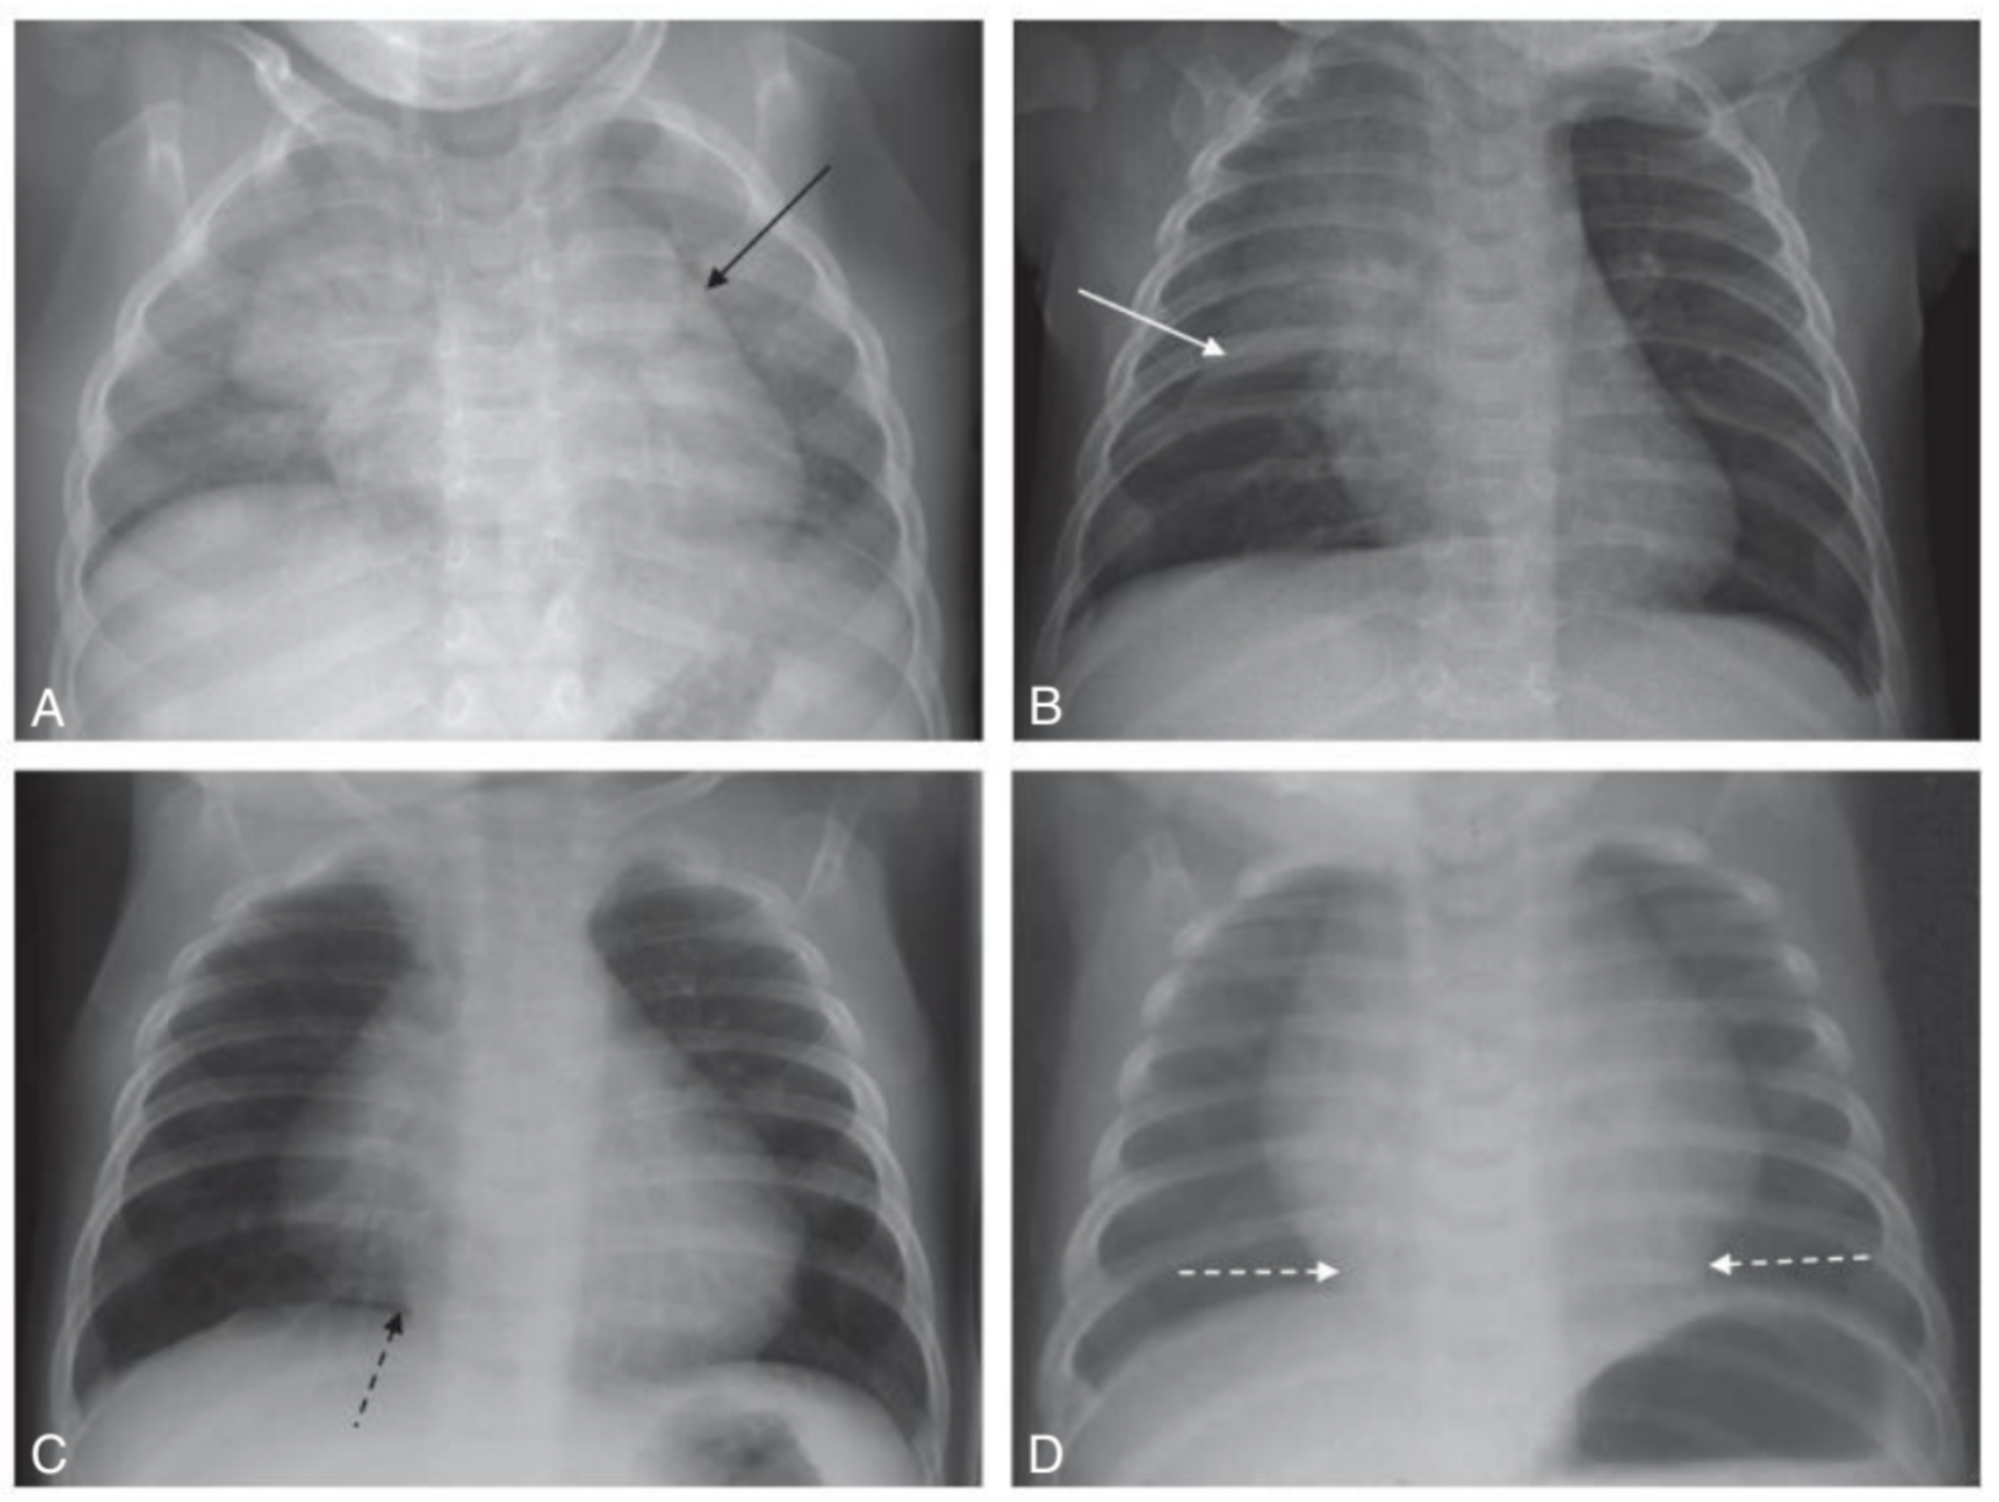
\includegraphics[width=0.6\textwidth]{thymus_enfant.png}
                    \caption{Les variations de l’image du thymus chez l’enfant}\label{fig:thymus}
                \end{figure}
                Aspects radiographiques normaux du thymus : aspect ondulé des bords du thymus sur un cliché réalisé en expiration (flèche noire) (A),aspect en voile latine (flèche blanche) (B), extension du thymus jusqu'à la coupole diaphragmatique (flèche noire en pointillés) (C),fausse impression de cardiomégalie du fait de l'extension inférieure du thymus (flèches blanches en pointillés) (D).	
                \item non visibilité du crosse aortique.
                \item portion antérieure du gril costal entièrement cartilagineuse, donc non visible sur la radiographie.
                \item courbure claviculaire accentuée du fait de la position des bras au-dessus de la tête.
                \item point d'ossification huméral supérieur.
                \item Déviation trachéale:
                \begin{figure}[H]
                    \centering
                    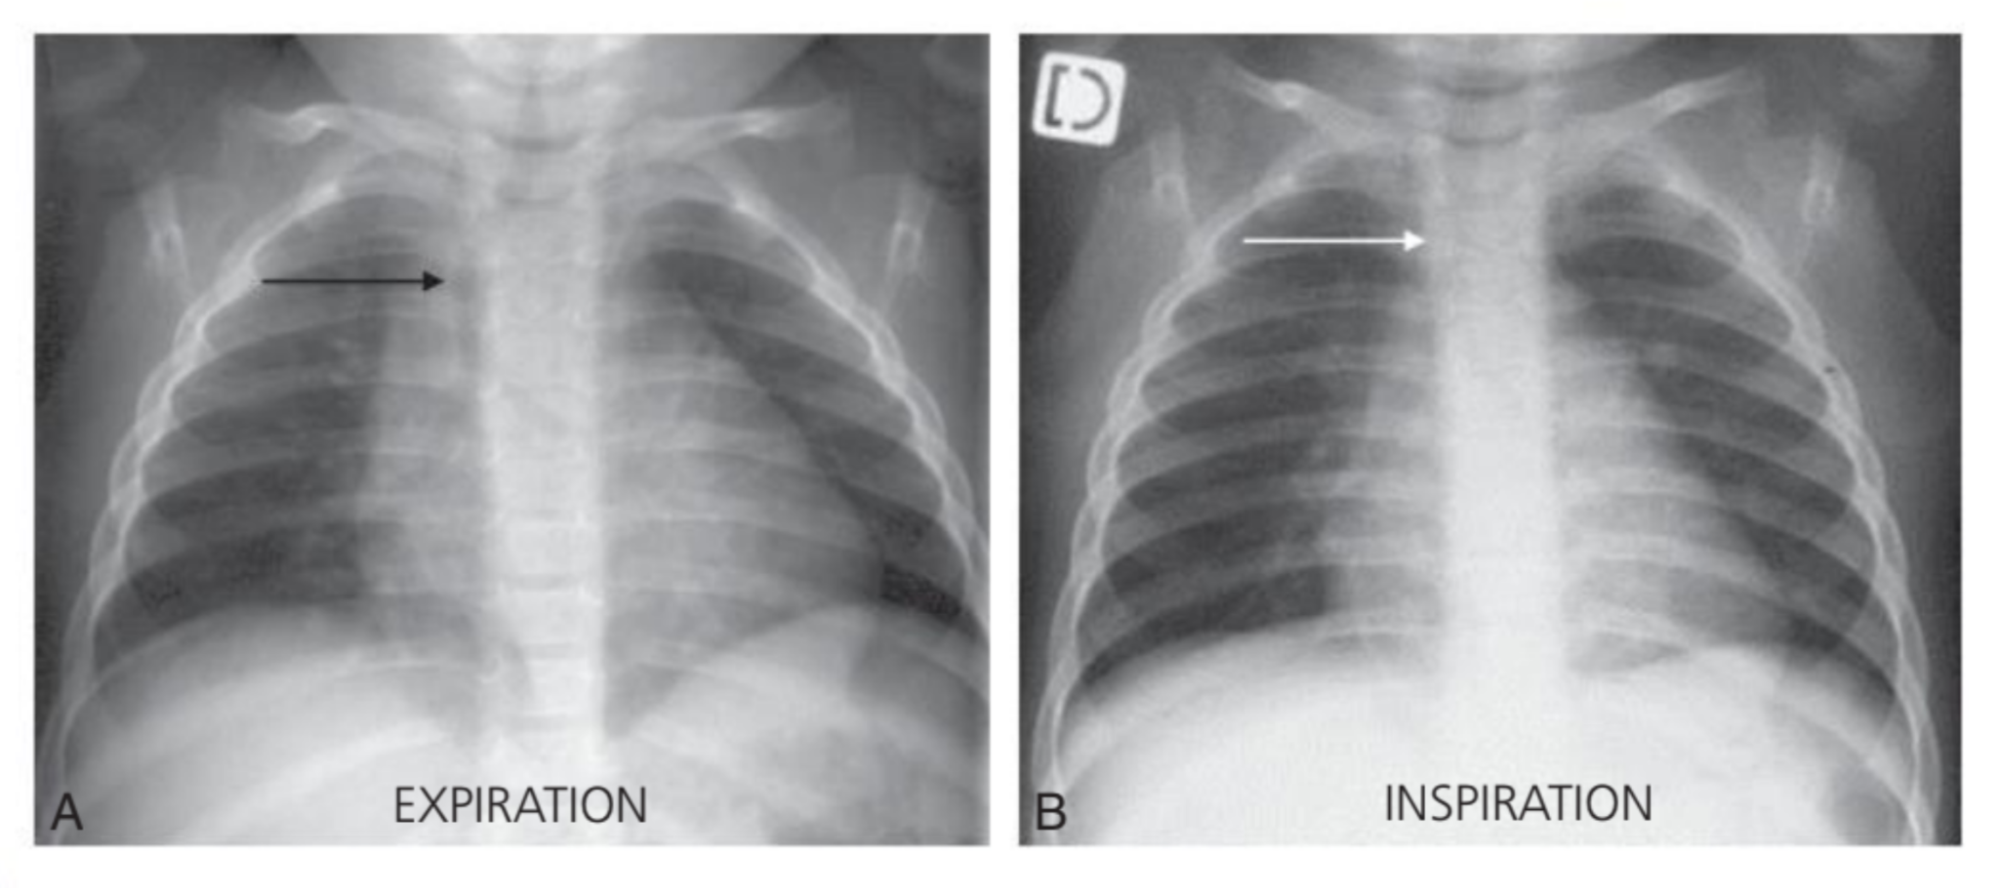
\includegraphics[width=0.6\textwidth]{tracheal.png}
                    \caption{La deviation trachéale}\label{fig:tracheal}
                \end{figure}
                Déviation trachéale physiologique vers la droite chez un nourrisson de 20 mois sur une radiographie de thorax réalisée en expiration (flèche noire) (A). Sur le cliché en inspiration, la trachée redevient rectiligne (flèche blanche) (B).
                \item L'incidence:\newline
                L'incidence de face en inspiration est suffisante dans la majorité des cas.
                Chez le petit enfant, elle est réalisée en incidence antéro-postérieure, puis en incidence postéro-antérieure lorsque l'enfant devient coopérant (après 4 ans environ).
                Chez le nouveau-né et le petit nourrisson ne tenant pas assis, l'examen est réalisé en décubitus dorsal.

            \end{enumerate}

            \subsubsection{La partie informatique de la problématique}\label{partie_info}
                Dans notre projet on veut crée un produit qui pourrait atténuer le flot des clichés thoraco pulmonaire qui doivent être traités individuellement par les radiologues, et en particuliérement les radiographies pédiatriques qui n'ont pas assés d'attention que les radiographies adulte, mais suivant une liste des anomalies predéfinie ou plutôt imposé par les base données publique à l'utilisation des étudiants, la liste des anomalies et la suivante:

                Dans notre projet, nous voulons créer un produit capable de réduire le flux de radiographies thoraco-pulmonaires, que les radiologues doivent traiter séparément. Anomalies, listes d'anomalies mandatées ou imposées par les bases de données publiques à l'usage des étudiants,  et ce qui suit:
                \begin{multicols}{2}\label{list_dia}
                    \begin{enumerate}
                        \item Aucun résultat
                        \item Élargissement cardio-médiastinal
                        \item Cardiomégalie
                        \item Opacité pulmonaire
                        \item Lésion pulmonaire
                        \item Œdème
                        \item Consolidation
                        \item Pneumonie
                        \item Atélectasie
                        \item Pneumothorax
                        \item Épanchement pleural
                        \item Autre lésions pleurales 
                        \item Fracture
                        \item Appareils de soutien
                    \end{enumerate}
                \end{multicols}

                Pour plus de detail sur la liste des anomalies voir la sous-section \ref{chexpertDB}.

        \subsection{Etat d'art}
            \subsubsection{Modèles de détection automatiques de pathologies thoraciques précise chez l‘adulte}
            La dernière décennie a vu la réalisation de plusieurs applications de l'IA sur la radiographie standard et plus particulièrement la radiographie thoracique, notamment chez l'adulte.
            Ces applications ont inclus 
            
            soit la détection automatique de motifs en relation avec des anomalies thoraco-pulmonaires par exemples les études suivantes:
            
            soit la détection de pathologies thoraco-pulmonaires précises telles que:
            
            \begin{itemize}[label=$\bullet$]
                \item La détection des lésions tuberculeuses pulmonaires
                \hspace*{1cm}Les algorithmes d'IA peuvent être des outils de triage très précis et utiles pour la détection de la tuberculose dans les régions à forte prévalence.
                \item La détection précoce des lésions du cancer du poumon
                \hspace*{1cm}L'algorithme d'IA peut améliorer les performances des lecteurs pour la détection des cancers du poumon sur les radiographies pulmonaires lorsqu'il est utilisé comme second lecteur.
                \item Récemment le diagnostic du SDRA et pronostic des patients atteints de COVID-19
                \hspace*{1cm}Schéma d'évaluation par radiographie pulmonaire assisté par intelligence artificielle pour COVID-19
            \end{itemize}

            \subsubsection{Modèles de détection de Pathologies précises ou d‘anomalies à la rx thoracique chez la Population Pédiatrique}

                Sur 29 ensembles de données de radiographie pulmonaire accessibles au public, 2 ensembles de données ne comprenaient que des radiographies pulmonaires pédiatriques et 7 ensembles de données comprenaient à la fois des patients pédiatriques et adultes. 

                Padash et al.ont identifié 55 articles mettant en œuvre un modèle d'IA pour l'interprétation des radiographies thoraciques pédiatriques ou des radiographies thoraciques pédiatriques et adultes. La classification des radiographies pulmonaires comme pneumonie était l'application la plus courante de l'IA, évaluée dans 65 \% des études. Bien que de nombreuses études rapportent une précision diagnostique élevée, la plupart des algorithmes n'ont pas été validés sur des ensembles de données externes.

        \subsection{Solution Proposée}\label{Solution_prop}
            Les  données de la population pédiatrique sont beaucoup moins documentées que celles de la population adulte, et notamment pour les radiographies thoraciques, ce qui nous inspirer pour créer ou collecter notre propre base de données, toujours en respectant la liste des anomalies déjà citées dans la sous-section \ref{list_dia}.
            La solution proposée se compose essentiellement de trois unités principales qui sont bien connectées les unes aux autres pour former un flux de travail fluide et solide.
            \begin{figure}[H]
                \centering
                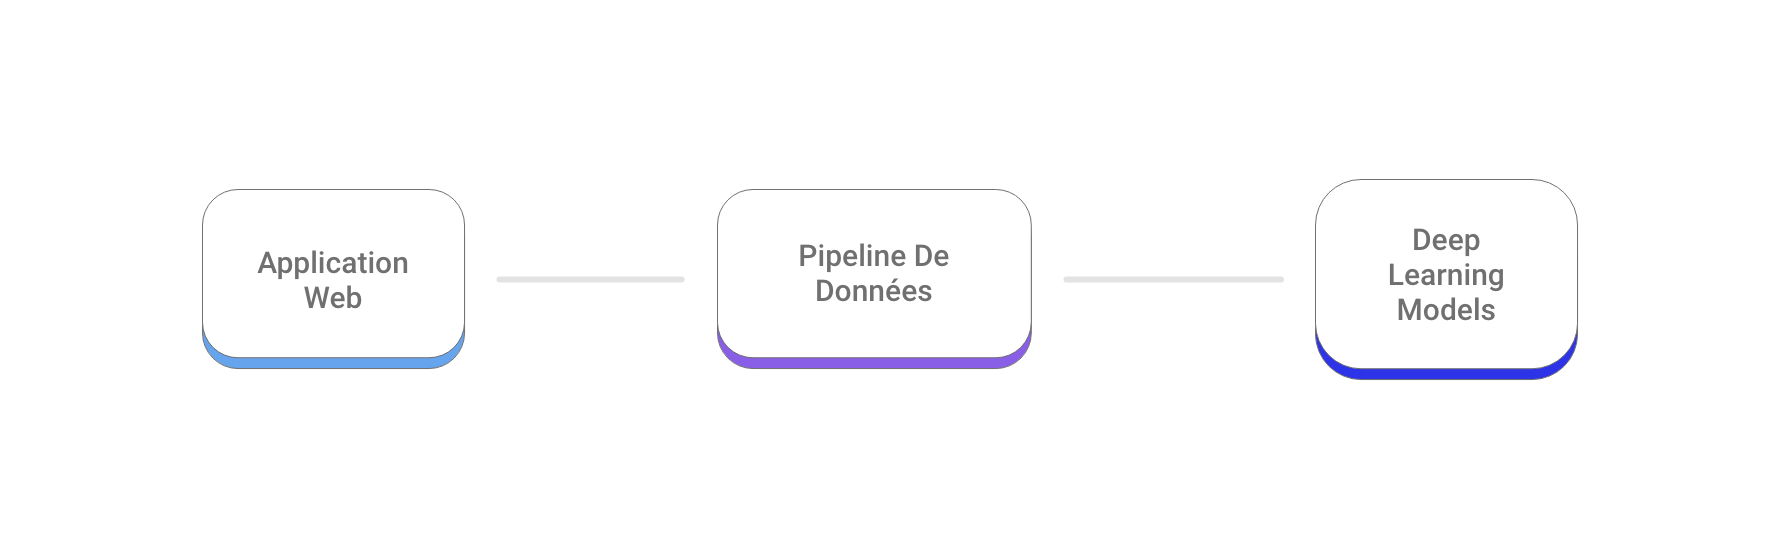
\includegraphics[width=1\textwidth]{sol_prop.jpg}
                \caption{Architecture générale du solution proposé}\label{fig:sol_prop}
            \end{figure}
            \subsubsection*{Application Web}
                Premiére phase:
                Une application web qui peut collecter des données. La collecte est effectuée par les collaborateurs voir sous-section \ref{Collaborateurs}. L'application doit être simple, légère, rapide et claire avec une interface concise direct afin de ne pas prendre beaucoup de temps au médecin.
            \subsubsection*{Pipline de données}
                Deuxiéme phase:
                Étant donné que le pipeline de données sera dans une phase de pré-apprentissage, nous devons préparer une base de données bien structurée et propre où toutes les valeurs sont définies et non nulles.
            \subsubsection*{Les modeles d'apprentissage en profondeur}
                Troisiéme phase:
                Construisez des modèles d'apprentissage en profondeur qui peuvent pré-diagnostiquer les anomalies dans le thorax osseux à partio des clichés thoraciques pédiatrique.


    \section*{Conclusion}
    En conclusion, voici quelques réflexions générales sur le projet et sur ce que vous devez faire pour pouvoir créer un projet capable d'effectuer  des pré-diagnostiques des radiographies pulmonaires pédiatriques.
    \begin{enumerate}
        \item Création d'une base de données pédiatrique étiquetée suivant la liste \ref{list_dia}
        \item Création d'un pipline de données pour prétraitement des données
        \item Création des modèles d'apprentissage en profondeur
    \end{enumerate}
    Cependant, afin de poursuivre le projet, nous devons d'abord savoir ce qu'est  l'apprentissage en profondeur.